\chapter{Methodology}

\section{Database Construction}

All available image quality benchmark databases are only suitable for evaluating the quality of images as a whole and not able to investigate which parts of the testing image contribute to the testing results or the score for a particular patch of image. 
In this project, we set up an experimental database to evaluate the quality that human perceive for each image patch.

\subsection{Testing image database}

A good database for testing is critical to be the success of the research. 
Due to the research orientation for video encoding, testing images are cropped from extracted frames in the video test sequence and noise types are added to the original video by H265/HEVC compression before extracting. 
In this database, we randomly select several patches from each image so that the database includes at least three attributes: smooth texture, complex texture and edge texture.

\begin{figure}[H]
  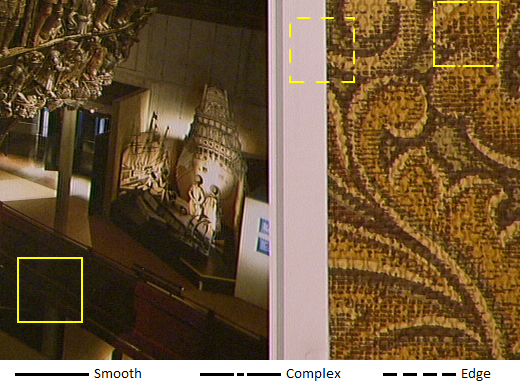
\includegraphics[width=\linewidth]{figures/imgpatches.png}
  \caption{Selected image patch.}
  \label{fig:selected-patch}
\end{figure}

\subsection{Database creation}

There are 40 original source videos of high-definition (1280x720) and full high-definition (1920x1080) being compressed by H.265/HEVC with different Quantization parameters (QPs) with the range from 2 to 50. Testing images are extracted from those testing video sequences. For each video sequence, we select a different number of frames depend on the original video, this number drops in the values from 5 to 15. After that, we select random positions of the image to crop different 128x128 patches of each pair of image. We also crop the center 64x64 patches from the original pair 128x128 to evaluate in the experiments. Finally, we obtain 161,144 images: 40286 pairs of 64x64 patches and 40286 pairs of 128x128 patches.


\begin{table}[H]
  \centering
  \begin{tabular}{| c | c | c | c | c | c | c | c |}
    \hline                          & \multicolumn{7}{c|}{QP} \\ \cline{2-8} 
    \multirow{-2}{*}{Orignal} & 25    & 30   & 35   & 40   & 45   & 50   & 55   \\ \hline 
    &&&&&&&\\
    
\includegraphics[height=1cm]{figures/11.png}                                                 &      &      & 
\includegraphics[height=1cm]{figures/12.png}       & 
\includegraphics[height=1cm]{figures/13.png}       & 
\includegraphics[height=1cm]{figures/14.png}    & 
\includegraphics[height=1cm]{figures/15.png}    & 
\includegraphics[height=1cm]{figures/16.png}    \\ 
    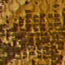
\includegraphics[height=1cm]{figures/21.png}                                                  &       &      &  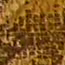
\includegraphics[height=1cm]{figures/22.png}     &  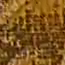
\includegraphics[height=1cm]{figures/23.png}     &  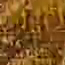
\includegraphics[height=1cm]{figures/24.png}     &  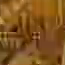
\includegraphics[height=1cm]{figures/25.png}     &  
\includegraphics[height=1cm]{figures/26.png}     \\ 
    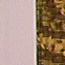
\includegraphics[height=1cm]{figures/31.png}                                                  & 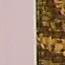
\includegraphics[height=1cm]{figures/32.png}     & 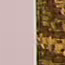
\includegraphics[height=1cm]{figures/33.png}    & 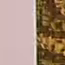
\includegraphics[height=1cm]{figures/34.png}    & 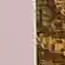
\includegraphics[height=1cm]{figures/35.png}    & 
\includegraphics[height=1cm]{figures/36.png}    &      &      \\ \hline
  \end{tabular}
  \caption{Example of testing image database.}
  \label{tab:exid}
\end{table}

\subsection{Testing methodology}

Depending on the nature of the test, observers may be expert or non-expert. Studies have found that systematic differences can occur between different laboratories conducting similar tests \cite{Bt2002}. One of the reasons for this is that expert observers have different view in compare with no-experts. Other explanations may include gender, age, and occupation. However, in reality, the majority of consumers should be non-expert observers are chosen for this experiment. Before final selection, all candidates have been checked to ensure that they possess normal visual acuity.

For the purpose of this experiment, 1200 subjects who are undergraduates, graduates, researchers, and lecturers of University of Fire Fighting and Prevention are employed. These subjects have been trained and practiced quality assessment of several sample images.

For the purpose of subject testing methodology, the International Telecommunication Union set the ITU-R BT.500-11 \cite{Bt2002} standard. In such standard, there are several popular subjective methodologies for testing such as Single stimulus categorical rating, Double stimulus categorical rating, Ordering by force-choice pairwise comparison and Pairwise similarity judgments. Double stimulus categorical rating is chosen in this practical. In this method, both the test and reference images are displayed for a fixed amount of time. After that, the images disappear from the screen and observers are asked to rate the quality of the test image according to the abstract scale containing one of the five categories: excellent, good, fair, poor or bad. All those images are displayed randomly. At the beginning of each session, an explanation is given to the observers about the type of assessment, the grading scale, the sequence and timing (reference image, grey, test image, voting period).

The previous image quality assessment methods are only suitable for assess quality of image as a whole. It cannot be directly applied for our testing experiments. Therefore, we modify this image selection method in the standard so that the users can only concentrate and assess the local image patch instead of the whole image. Each pair quality is assessed with the following procedure: The subjects observe the original image within the time T1 at minimum 5s then click on the observing image patch to observe the compressed image within the time T2. After watching at least twice per image, the observers would score on scale of 5 as in Fig.\ref{fig:testing-software}.

\begin{figure}[H]
  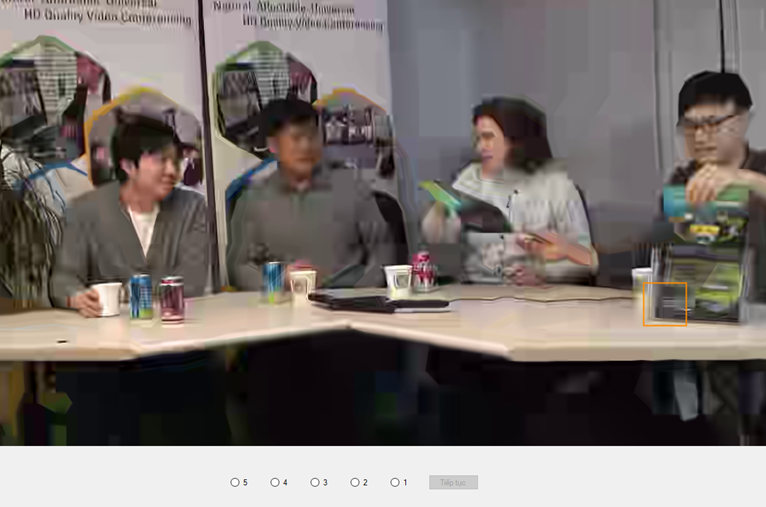
\includegraphics[width=\linewidth]{figures/softtest.png}
  \caption{Testing software screenshot.}
  \label{fig:testing-software}
\end{figure}

At the end of experiment, each pair is scored by the mean of the DMOS that up to 20 subjects give during the experiment.

We carefully select 1511 pairs which are scored by at least 10 people and name this sub-database HMII (Human Machine Interaction Image). HMII is used to evaluate well-known IQA algorithms and our methods in the second contribution. 

\subsection{Benchmark Analyses}

To analyze the efficiency of IQA algorithms, we apply 7 state-of-the-art full reference image quality assessment
methods on the proposed HMII database, to investigate
their performance and demonstrate the new challenges in
fine-grained image-patch quality assessment problem. The FR-IQA algorithms include PSNR, SSIM \cite{Wang2004}, RFSIM \cite{Zhang2010}, FSIM \cite{Zhang2011}, SRSIM \cite{Zhang2012}, UQI \cite{Wang2002}, VSI \cite{Zhang2014}. The implementations of all algorithms are obtained from the public websites. 

\section{Deep Image-Patch Quality Assessment}

\subsection{Architecture}

Being known as a designed architecture to learn the similarity relations between two given inputs, Siamese network has been applied for face verification \cite{Chopra2005} and signature \cite{BROMLEY2004} tasks. The main concept is processing two networks that share the same architecture and weights parallel. In this work, we employ Siamese network for feature extraction. Before feeding the extracted features as input to the regression layers, feature extraction is followed by a feature fusion step. The proposed architecture of DIPQA is sketched in Fig.\ref{fig:dipqa-architecture}

\begin{figure}[H]
  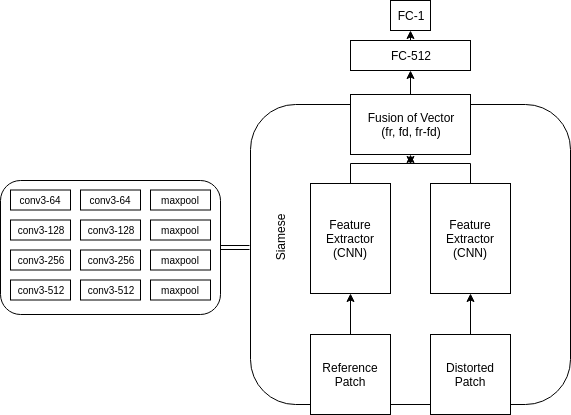
\includegraphics[width=\linewidth]{figures/dipqa.png}
  \caption{Deep Image-Patch Quality Assessment Network Architecture.}
  \label{fig:dipqa-architecture}
\end{figure}

With the successful adaptation for various computer vision tasks \cite{Girshick2015, Shelhamer2017}, especially in image quality assessment \cite{Bosse2018}, VGGnet \cite{Simonyan2014} was chosen as a base network for the feature extraction. The input of the VGG network is the size of 224 x 224 pixels. For the purpose of adjusting the network for 64 x 64 and 128 x 128 pixels, we have tried to change the architecture of VGG network such as: extend the network by 3 layers \cite{Bosse2018}, cut last 3 layers, last 6 layers or even replace VGG with Resnet. Finally, we choose to cut the last 3 layers of VGGnet and achieve the best performance comparing to the other approaches. Our VGGnet-inspired DCNN comprised 12 weight layers as a feature extraction module and a regression module. The features are extracted in a series of conv3-64, conv3-64, maxpool, conv3-128, conv3-128, maxpool, conv3-256, conv3-256, maxpool, conv3-512, conv3-512, maxpool, layers. The fused features are regressed by a sequence of two fully connected layers (FC-512, FC-1). This results in about 17.3 million trainable network parameters. All convolutional layers apply 3x3 pixel-size convolution kernels and are activated through a rectified linear unit (ReLu) \cite{Nair2010} activation function after being normalized with batch normalization. All max-pool layers have 2 x 2 pixel-sized kernels. In order to prevent overfitting, dropout regularization \cite{Sutskever2014} is applied to the fully connected layers with a ratio of 0.5.  

\subsection{Feature Fusion}

The feature extraction layers extract $f_r$ and $f_d$ which are the feature vectors of reference and distorted patch respectively. The regression layers require the network to combine these two vectors in a feature fusion step. A simplest strategy is concatenating $f_r$ and $f_d$ to an unique vector $(f_r,f_d)$. Beside, $f_r-f_d$ is known as a meaningful representation for distance in feature space. Therefore, concatenating $f_r-f_d$ is expected to contribute to learning to relations between reference and distorted patch. The final output of this state is $(f_r,f_d,f_r-f_d)$

\subsection{Training Method}

For better convergence of the optimization, the feature extraction parameters are initialized with VGG13-batchnorm weights which is trained on ImageNet dataset. Our network is trained end-to-end by backpropagation, over a number of epochs. The adaptive moment estimation optimizer (ADAM) \cite{Kingma2015} is employed to alter the regular stochastic gradient descent method. Parameters of ADAM are chosen as recommended in \cite{Kingma2015} $\beta_1 = 0.9, \beta_2 = 0.999, \epsilon = 10^{-8}$ and the learning rate $\alpha$ is initially set to $5\times10^{-4}$. The mean loss, PCC, SRCC over images during validation is computed in evaluation mode after each epoch.